\chapter{Introduction}
\label{chap:introduction}

The global flow of foreign direct investment (FDI) has risen from almost nothing
in the 1970s to over \$2.3 trillion dollars in 2016, becoming an important
source of global capital (Figure~\ref{fig:globalfdi}). For developing countries
especially, capital from multinational corporations (MNCs) is robust to global
economic downturns, prompting major international organizations to endorse FDI
as a key factor to economic development and poverty reduction
\citep{Mallampally1999, WorldEconomicForum2013}.\footnote{While FDI into
  developed economies dropped almost 50\% during the 2000 recession and the 2008
  financial crisis, FDI into developing countries only experienced a plateau or
  a small reduction. More recently, as global FDI flow slipped in 2016 and 2017,
  FDI into developing countries still remained stable \citep{UNCTAD2018}.} Within the scholarly
field of International Political Economy (IPE), much of the literature starts
with the view that countries will always seek FDI for its various benefits
\citep{Jensen2008b}. Works in IPE tend to focus on \textit{how} countries can
attract FDI, and do not question \textit{whether} they want to do so
\citep{Jensen2003, Li2003, Li2006, Ahlquist2006}.\footnote{Two recent exceptions
  are \citet{Pinto2013} and  \citet{Pandya2016}, who are the first to examine variation in
  countries' demand for FDI.}

\begin{figure}[tbp]
  \centering
  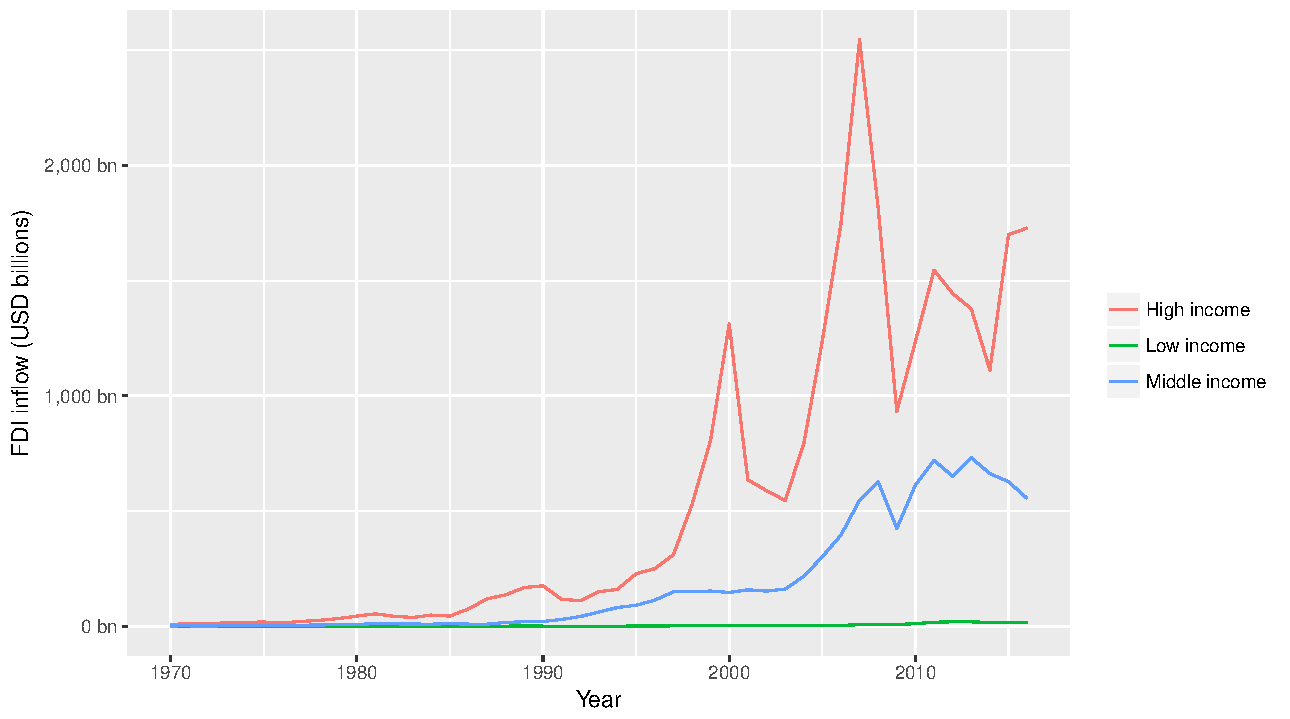
\includegraphics[width=0.8\textwidth,keepaspectratio]{../figure/global_fdi}
  \caption[FDI global inflow, 1970-2006.]{FDI global inflow, 1970-2006. The last
    four decades witness the growth of FDI into the most important source of
    global capital. Source: World Bank's World Development Indicators.}
  \label{fig:globalfdi}
\end{figure}

However, such an assumption is no longer tenable given the mounting evidence
that not all FDI are the same and that its effects are highly conditional.
Whether countries benefit from FDI depends on the sophistication of their labor
force, the technical capability of their domestic business, and various
government policies. Indeed, reviewing the vast yet inclusive literature on the
effects of FDI, \citet{Lipsey2005} suggest ``the main lesson might be that the
search for universal relationships [between FDI and host country economic
performance] may be futile.''

If the effects of FDI are so conditional, it is unreasonable to assume that
countries' preference for FDI is homogeneous. By holding this assumption, we
neglect the role of the state in shaping global capital flow, falling prey to
the discredited ``race to the bottom'' thesis of globalization
\citep{Mosley2005}. Indeed, even in the face of footloose capital and
transnational actors, different governments still offer different combinations
of policy choices especially crafted for their constituencies, \`a la Tiebout.
As governments maintain substantial autonomy and variation in the realm of
fiscal, social, and environmental policies, there is no reason to believe that
FDI policies are somehow uniform across the globe.

Arguably, political scientists should be dissatisfied with the current
literature on the political determinants of FDI. The status quo often involves adding a
political variable to an existing economic model of FDI and checking for its
effect. In this approach, states are just billiard balls of different shapes and
size for MNCs to pick and choose, and left unpacked is the effect of internal
politics on FDI policies. Furthermore, even if we only care about MNCs'
preference with regards to countries' characteristics, to get an accurate
estimate we must still take into account countries' preference. For example,
take the received wisdom that democracies receive more FDI \citep{Jensen2008a}.
Without taking into account countries' preferences, it is difficult to interpret
this finding as democracies actively pursuing MNCs or as MNCs finding
democracies attractive.

\section{Goal of the research}

My research aims to estimate the preference of countries and MNCs for each
other. I develop an empirical strategy that takes into account the two-sided
nature of the FDI market, i.e. a subsidiary can only materialize if both the MNC
and the host government agree. Recognizing that this two-sided matching dynamics
can also be found in the labor or the marriage markets, I adapt the statistical
models first developed in Sociology for labor and marriage markets and apply
them to the study of FDI \citep{Logan1996, Logan2008}.

In doing so, I simultaneously address three long-standing issues in the FDI
literature. First, I ``bring the state back in,'' filling the gap in the
literature on the variation of countries' preference for
FDI.\footnote{\citet{Evans1985}'s book, ``Bringing the state back in,'' argues
  that states are weighty actors with their own capabilities and initiatives,
  and are not merely an arena for societal and interest groups to negotiate
  their share. Here, I argue that states are weighty actors with their own
  preferences regarding which MNC is allowed inside its border, and are not
  merely passive receivers of FDI.} Two notable exceptions are \citet{Pinto2013}
and \citet{Pandya2016}, whose pioneering works propose partisan politics and
regime types as factors shaping preferences for FDI. However, while their
theories are ground-breaking, the empirical estimation of countries' preference
remains inadequate. In addition, these researchers have not used their findings
to re-estimate the preference of MNCs and disentangle the ``push'' vs ``pull''
factors of FDI flow.\footnote{``Push factors'' refer to characteristics of the
  home country and of the MNC, pushing capital out from its origin. ``Pull
  factors'' refer to the characteristics of the host country, pulling capital
  towards its destination.} Using a two-sided matching model, I will naturally
be able to estimate both sides' preference.

Second, I pay more attention to countries' preference for different types of
FDI. While the IPE literature has largely focused on the quantity of FDI flow,
countries care deeply about its type. They use various incentives and
restrictions to target FDI that invests in a remote region, brings new
technology, or improves the balance of payment by exporting and bringing back
foreign currencies \citep{Ricupero2000}. For example, since 2006, China's
official FDI policy has been ``quality over quantity,'' promoting FDI with
intense R\&D in high-productivity sectors \citep{Guangzhou2011}. As
\citet{UNCTAD2015} proclaims, ``Today, increasing the quantity of investment is
not enough. What matters is its quality, i.e. the extent to which investment
delivers concrete sustainable development benefits.'' Two-sided matching model
can be used to estimate countries' preference for different types of FDI. Just
as it can estimate MNCs' utility function for countries' characteristics (e.g.
market size, level of development), two-sided matching model can estimate
countries' utility function for MNCs' types (e.g. technological sophistication,
export strategy).

Third, while the majority of the literature uses FDI flow data, these data are
accounting constructs created to keep track of countries' balance of payment.
They map poorly to concepts in Political Science theories. Very often, the
variable of interest in our theories is the scale of MNCs' activities in the
host country, which can be very different from the amount of border-crossing
capital thanks to MNCs' complex financial and tax strategies \citep{Kerner2014}.
Therefore, we would do much better testing our theories with firm-level
operational data. Because the two-sided matching model is a behavioral model in
which each actor's decision is a unit of observation, and we can naturally use
it to analyze firm-level data.

In sum, my dissertation benefits the field by using firm-level data to estimate
both firms' and countries' preference for each other's characteristics. In this
two-sided matching model, MNCs and countries evaluate their available options
according to their utility functions, choose the best alternative, culminating
in an MNC's subsidiary located in a host country.

Estimating this model would be straightforward if we could observe not only
subsidiaries' locations but also their set of options (called their
``opportunity set'' in the matching literature).\footnote{Discrete choice models
  can be used to estimate the utility function when both the choice and the set
  of options are observed. Indeed, discrete choice models remain the dominant
  empirical approach in the industrial location literature. However, by not
  taking into account the two-sided nature of the FDI market, these models
  assume that all countries are available as potential locations for all MNCs.
  Thus, to use discrete choice models in studying FDI location choice is to
  ignore the fact that not all MNCs have the same set of location options
  \citep{Arauzo-Carod2010}.} Unfortunately, while data on subsidiaries' location
are available, the opportunity set is generally unobserved as researchers cannot
peek into the negotiation process between countries and MNCs. The two-sided
matching model solves this problem by using the Metropolis-Hastings (MH)
algorithm, a Markov chain Monte Carlo (MCMC) approach that repeatedly samples
new opportunity sets and rejects them at an appropriate rate to approximate
their true distribution. In addition, the estimated preference parameters in the
two-sided model have a convenient interpretation as the relative weight of
different variables on MNCs' and countries' utility. This allows us to make
statements such as ``In evaluating MNCs, China values a 2\% increase in the
firm's capital as much as a 1\% increase in labor demand.''

\section{Relevance of the research to FDI policy formulation}

During my time at the World Bank, an official opined that many of his country
clients needed help with formulating their FDI attraction policies. Regardless
of their situations, most country clients want to increase their FDI inflow,
ideally in high-tech industries, relying on fiscal incentives such as tax
holiday, land concession, or lower utility price. Economists tend to look
askance at such heavy-handed industrial policy. Rather than encouraging
governments to pick winners, the World Bank gives governments the sanctioned
advice of getting the fundamentals right, i.e. liberalizing trade and
investment, upholding rule of law, eradicating corruption, and upgrading its
labor force. Perhaps not coincidentally, most of the FDI literature has also
focused on studying what country characteristics are attractive to MNCs,
settling on the same familiar list of desirables.

These two approaches to industrial policy veer towards the extremes, one
trusting and the other dismissive. At the same time, they are also similar. Both
neglect the fact that a country's FDI inflow depends not only on its policies
but also on the competitive landscape in which it is situated. In formulating their
FDI strategies, policy makers should neither solipsistically determine what
sectors they want, nor abstractly ask what macro conditions are associated with
FDI inflow. Rather, they are better off preparing strategically for realistic
scenarios. For example, given China's rising wage and tougher environmental
regulations, how much and what type of FDI will diversify out of China? What
share of that outflow can our country capture at the current condition? How much
can we capture if we improve our labor productivity by 5\% or 15\%? How much can
we capture if other countries also increase their GDP per capita by 10\% in the
mean time? Once I estimate MNCs' and countries' preference, I can simulate their
decisions under such scenarios, allowing policy makers to better strategize
their FDI attraction. To quote Sun Tzu's ``The Art of War'' (as the business
community is apt to do), ``If you know the enemy and yourself, you need not fear
the result of a hundred battles.''

In other words, my research gives policy makers the tool to formulate better
informed industrial policies. The time is right for such an approach. First, the
opportunity is there to target the FDI that China no longer attracts. As China
becomes more expensive, aims to move into high-tech manufacturing, and withdraws
their preferential treatment, MNCs are looking towards diversifying into other
countries. In 2013, an American lawyer in Phnom Penh said that ``Every couple
days, I'm getting calls from manufacturers who want to move their businesses
here from China'' \citep{Bradsher2013}. By 2017, a quarter of AmCham China's
survey respondents reported that they had either moved operations out of China
or were planning to do so, with nearly half moving to other parts of Asia
\citep{AmCham2018}.

Second, there has been a resurgent appetite for industrial policy at the World
Bank, the largest and most influential banker-cum-consultant for the developing
world. For a long time, World Bank economists disavow industrial policy so
completely that the East Asian miracle, arguably the clearest example of
state-led industrialization, was interpreted as the result of
``market-conforming'' policies \citep[355]{WorldBank1993}.\footnote{See
  \citet{Amsden1994} and \citet{Rodrik1994} for a forceful rebuttal. Indeed, the
  East Asian miracle, i.e. the rapid growth with equity of eight high-performing
  Asian economies (Hong Kong, Korea, Singapore, Taiwan, China, Indonesia,
  Malaysia, and Thailand), was a Rorschach test for the international
  development world. Looking at the same set of facts, some saw the state
  micro-manage the market, while others, like the World Bank, saw the state
  getting the macro conditions right.} However, since the appointment of Chief
Economist Justin Yifu Lin in 2008, the World Bank has supported programs that
aim to restructure the economy towards high-value added sectors
\citep{Wade2012}. These programs look like industrial policy, talk like
industrial policy, but are called ``Competitive Industries''
instead.\footnote{In an advertising brochure, the Competitive Industries
  practice describes itself as ``Going \textit{beyond macroeconomic reform
    agenda} to identify and address the \textit{real microeconomic barriers} to
  the growth of \textit{industries with high economic and social benefits}'' and
  ``\textit{Intervening aggressively} \ldots to enable those industries to seize
  their 'windows of opportunity' to grow, compete and generate inclusive,
  productive employment'' (emphasis added) \citep{WorldBank2011}. In recent
  years, the program has expanded into the ``Competitive Industries and
  Innovation Program,'' a multi-donor partnership with the support of the World
  Bank, the European Union, and several donor governments. ``Industrial policy''
  may still be a taboo at the World Bank, but ``competitiveness'' and
  ``innovation'' are fully embraced as they hide the state and highlight the
  private sector.} Purists at the World Bank may remain skeptical, but
operational economists and specialists are understandably onboard. Their daily
job is to provide country clients with money and advice on how to spend
it---there is no wonder why they warmly support a development strategy based on
targeting specific industries. Effective or not, such a development program
happens to provide ample opportunities for lucrative advice-giving. Today, ten
years after the first sign of resurgence, the support for industrial policy has
become mainstream albeit under other names. Indeed, the director of Trade and
Competitiveness, one of the World Bank's 14 global practices, recently exclaimed
in an official blog post, ``FDI matters, but not all FDI is created equal,'' and
promised to help countries target the ``right'' kind of FDI \citep{Fruman2016}.

\section{Roadmap}

The rest of my research project proceeds as follows. In
Chapter~\ref{chap:literature_issues}, I review in-depth the three issues in the
literature of FDI's political determinants, outlining the current attempts to
address them and how my approach can contribute to the solution. In
Chapter~\ref{chap:model}, I describe the two-sided matching model, including
both its game-theoretic origin and its statistical estimation.
Chapter~\ref{chap:simulation} uses simulation and US labor data to demonstrate
the correctness of the model and explore its characteristics.
Chapter~\ref{chap:FDI} brings us back to the study of FDI, applying the model on
firm-level data of Japanese MNCs in East and Southeast Asia.
Chapter~\ref{chap:conclusion} explores potential improvements and other
applications of the two-sided matching model in different areas of Political
Science.

%%% Local Variables:
%%% mode: latex
%%% TeX-master: "AnhLe_dissertation.tex"
%%% End:
